\section{Хроматическое число и хроматический индекс графа. Теорема о хроматическом числе графа в 
простейших случаях. Теорема о четырех красках. Найти хроматическое число графа. Ответ 
обосновать.}

\begin{definition}
    \textit{Раскраской графа (вершинной раскраской, правильной
    вершинной раскраской)} называется такое приписывание цветов вершинам
    графа, что смежным вершинам сопоставляются разные цвета.
\end{definition}

\begin{definition}
    Граф называется \textit{n-раскрашиваемым},
    раскраска графа, использующая n цветов.
\end{definition}

\begin{definition}
    Хроматическим числом графа $\chi(G)$ называется минимальное
    количество цветов в раскраске этого графа.
\end{definition}

\begin{theorem}
    Оценка хроматического числа графа в простейших случаях.
    \begin{enumerate}[left=0.0em, labelsep=1em, topsep=0.0em, itemsep=0pt, parsep=0.5em]
        \item $\chi(G)=1$ тогда и только тогда, когда граф не содержит ни одного ребра;
        \item $\chi(G)=2$ тогда и только тогда, когда $G$ -- двудольный граф, содержащий хотя бы одно ребро;
        \item если $G$ -- дерево, содержащее хотя бы одно ребро, то $\chi(G)=2$;
        \item если $K_n$ -- полный граф, то $\chi(K_n)=n$;
        \item если в графе есть полный подграф $K_s$, то $\chi(G) \geq s$.
    \end{enumerate}
\end{theorem}

\begin{proof}
    Оценка хроматического числа графа в простейших случаях.
    \begin{enumerate}[left=0.0em, labelsep=1em, topsep=0.0em, itemsep=0pt, parsep=0.5em]
        \item Если в графе нет рёбер, то всем вершинам можно приписать один цвет.
        \item Вершины из одной доли раскрашены в один цвет и не смежны по определению.
        Доли всего две, следовательно, $\chi(G)=2$.
        \item Дерево -- двудольный граф без циклов. Аналогично 2, $\chi(G)=2$.
        \item Так как все вершины графа смежные, то им необходимо сопоставить
        разные цвета.
        \item В полном графе на $n$ вершинах, можно выделить полный подграф
        $n-1$. $\chi({G}')=n-1$ для подграфа, $\chi(G)=n$ для самого графа. Тогда $n \geq n - 1$. 
    \end{enumerate}
\end{proof}

\newpage
Одной из основных теорем математики являются теорема о \textbf{четырёх красках}.
Очень долго она была гипотезой, но сейчас считается теоремой.

Пусть есть некоторая карта государств, при этом два государства называются
соседними, если они имеют общую границу.

\begin{theorem}
    Пусть каждое государство является односвязной областью, соседние
    государства имеют протяжённую границу. Тогда их можно раскрасить,
    используя не более 4 цветов так, чтобы соседние государства были
    раскрашены в разный цвет.

    Рассмотрим столицы этих государств. Им сопоставим вершины графа. Если
    страны являются соседними, то соединим вершины, соответствующие их
    столицам, рёбрами. Тогда теорему можно сформулировать следующим
    образом:
\end{theorem}

\begin{theorem}
    Хроматическое число планарного графа не больше четырех.
\end{theorem}

\begin{proof}
    Теорема была доказана в 1978 году с помощью ЭВМ и пока не имеет
    доказательства в традиционном понимании.
\end{proof}

\textbf{Алгоритм последовательной раскраски:}
\begin{enumerate}[left=0.0em, labelsep=1em, topsep=0.0em, itemsep=0pt, parsep=0.5em]
    \item Упорядочиваем вершины графа $G$ в порядке невозрастания степеней --
    от вершин максимальной степени к минимальной.
    Получаем последовательность L.
    \item Полагаем цвет окраски p=1.
    \item Если список L пуст, то останавливаемся. Если нет, то переходим к шагу
    4.
    \item Окрашиваем в цвет p первую вершину из списка L и все вершины,
    которые не смежны с вершинами, уже окрашенными в цвет p, рассмотрение
    этих вершин производим в порядке, в котором они находятся в
    последовательности L. После того, как вершина получила цвет, удаляем ее из
    списка. После рассмотрения всех вершин последовательности р:=p+1.
    Переходим к шагу 3.
\end{enumerate}

\newpage
Пример раскраски на графе.
\begin{figure}[h]
    \centering
    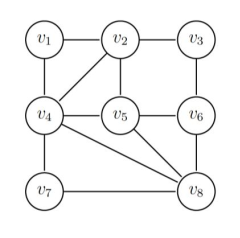
\includegraphics[scale=0.5]{34_1.png}
\end{figure}
\begin{figure}[h]
    \centering
    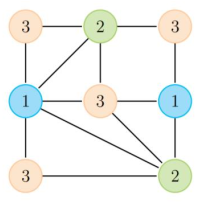
\includegraphics[scale=0.5]{34_2.png}
\end{figure}

Очевидно, что раскраска оптимальна, так как в графе есть подграф $K_3$,
и следовательно, $\chi(G) \geq 3$.

\begin{definition}
    \textit{Рёберной раскраской графа} называется приписывание рёбрам
    цветов так, чтобы рёбра, имеющие общую вершину, были раскрашены в
    разные цвета.
\end{definition}

\begin{definition}
    \textit{Хроматическим индексом графа} называется минимальное
    количество цветов в реберной раскраске графа.
\end{definition}

\begin{theorem}
    Хроматический индекс графа равен $\delta$ или $\delta+1$, где
    \begin{align*}
        \delta = \max \delta(v), v \in V.
    \end{align*}
\end{theorem}